\chapter{Background and Related Work}

\section{Hierarchical Task Networks}

HTN is a paradigm in AI planning for automated planning. Classical planning focuses on finding sequence to get from point A to point B, while HTNs focus on high-level decomposition until high-level tasks become manageable, primitive subtasks \parencite{nau_shop_1999}. Four key components within HTN are tasks, methods, initial state and a goal. Tasks are the \emph{what} of the plan. Primitive tasks are basic actions that can be executed in the environment. Non-primitive tasks are compound tasks, these are high-level tasks composed of several primitive tasks. Methods are the \emph{how} and are the recipe telling the planner how to decompose a specific task into sub-tasks. The initial state describes the state that is to be planned for and holds information about the world at the beginning before planning starts. Decomposition is done recursively by the planner and stops when it has found a task set that can be directly performed by \emph{planning operators}. The goal serves as the starting point for planning, which the planner then processes by assigning simple tasks in the task tree if conditions of the task are met. A task tree is the representation used by HTNs which contains all primitive and compound tasks in a hierarchy. Decomposition takes place when a compound task in the tree is reached during planning, which is then solved by a method that can fulfill the conditions and assigns simple tasks as defined in the method. Figure~\ref{fig:generic-htn} illustrates a simple example of a generic HTN with simple tasks $t1,.., t5$ and compound tasks $T1, T2$ which would then be decomposed using methods $m1, m2, m3$.

% Generic HTN tree (top-down) -- include with % Generic HTN tree (top-down) -- include with % Generic HTN tree (top-down) -- include with \input{chapters/generic_htn}
% Uses the compound/primitive/method styles and \htnpre from main.tex
\begin{figure}[htbp]
  \centering
  \begin{forest}
    for tree={
      font=\small, align=center, inner sep=3pt, rounded corners=2pt,
      minimum width=1.0cm, minimum height=0.7cm,
      l sep=0.9cm, s sep=0.5cm,
      edge={draw=black!60, thick},
      parent anchor=south, child anchor=north,
    }
    [{$T_1$}, compound
      [{$m_1$\htnpre{$p_1$}}, method
        [{$t_1$}, primitive]
        [{$T_2$}, compound
          [{$m_2$\htnpre{$p_2$}}, method
            [{$t_2$}, primitive]
          ]
          [{$m_3$\htnpre{$\neg p_2$}}, method
            [{$t_3$}, primitive]
            [{$t_4$}, primitive]
          ]
        ]
        [{$t_5$}, primitive]
      ]
    ]
  \end{forest}

  \medskip
  % Legend
  \begin{tikzpicture}[font=\scriptsize,
      every node/.style={inner sep=2pt, rounded corners=2pt}]
    \node[draw, double, fill=blue!8] (c) {compound task};
    \node[draw, fill=white, right=6pt of c] (p) {primitive task};
    \node[draw, dashed, fill=orange!8, right=6pt of p] (m) {method (with precondition)};
  \end{tikzpicture}

  \caption{Generic hierarchical task network.}
  \label{fig:generic-htn}
\end{figure}

% Uses the compound/primitive/method styles and \htnpre from main.tex
\begin{figure}[htbp]
  \centering
  \begin{forest}
    for tree={
      font=\small, align=center, inner sep=3pt, rounded corners=2pt,
      minimum width=1.0cm, minimum height=0.7cm,
      l sep=0.9cm, s sep=0.5cm,
      edge={draw=black!60, thick},
      parent anchor=south, child anchor=north,
    }
    [{$T_1$}, compound
      [{$m_1$\htnpre{$p_1$}}, method
        [{$t_1$}, primitive]
        [{$T_2$}, compound
          [{$m_2$\htnpre{$p_2$}}, method
            [{$t_2$}, primitive]
          ]
          [{$m_3$\htnpre{$\neg p_2$}}, method
            [{$t_3$}, primitive]
            [{$t_4$}, primitive]
          ]
        ]
        [{$t_5$}, primitive]
      ]
    ]
  \end{forest}

  \medskip
  % Legend
  \begin{tikzpicture}[font=\scriptsize,
      every node/.style={inner sep=2pt, rounded corners=2pt}]
    \node[draw, double, fill=blue!8] (c) {compound task};
    \node[draw, fill=white, right=6pt of c] (p) {primitive task};
    \node[draw, dashed, fill=orange!8, right=6pt of p] (m) {method (with precondition)};
  \end{tikzpicture}

  \caption{Generic hierarchical task network.}
  \label{fig:generic-htn}
\end{figure}

% Uses the compound/primitive/method styles and \htnpre from main.tex
\begin{figure}[H]
  \centering
  \begin{forest}
    for tree={
      font=\small, align=center, inner sep=3pt, rounded corners=2pt,
      minimum width=1.0cm, minimum height=0.7cm,
      l sep=0.9cm, s sep=0.5cm,
      edge={draw=black!60, thick},
      parent anchor=south, child anchor=north,
    }
    [{$T_1$}, compound
      [{$m_1$\htnpre{$p_1$}}, method
        [{$t_1$}, primitive]
        [{$T_2$}, compound
          [{$m_2$\htnpre{$p_2$}}, method
            [{$t_2$}, primitive]
          ]
          [{$m_3$\htnpre{$\neg p_2$}}, method
            [{$t_3$}, primitive]
            [{$t_4$}, primitive]
          ]
        ]
        [{$t_5$}, primitive]
      ]
    ]
  \end{forest}

  \medskip
  % Legend
  \begin{tikzpicture}[font=\scriptsize,
      every node/.style={inner sep=2pt, rounded corners=2pt}]
    \node[draw, double, fill=blue!8] (c) {compound task};
    \node[draw, fill=white, right=6pt of c] (p) {primitive task};
    \node[draw, dashed, fill=orange!8, right=6pt of p] (m) {method (with precondition)};
  \end{tikzpicture}

  \caption{Generic hierarchical task network.}
  \label{fig:generic-htn}
\end{figure}


To find a plan that is suitable for a given initial state and an HTN tree, there are several planners which can be used, e.g.\ probabilistic \parencite{sherkat_two_2025} or heuristics \parencite{georgievski_htn_2015}. Two planners that serve as a starting point for an introduction into this subject are SHOP and SHOP2 \parencite{nau_shop_1999, nau_shop2_2003, nau_applications_2005}. SHOP is ``Simple Hierarchical Ordered Planner'' which decomposes tasks recursively into directly executable primitive tasks exactly in the order they are to be executed. This significantly reduces complexity in the decision making for task sequences because the planner knows at each step the current state of the world, thus removing uncertainty in planning. SHOP2 adds the possibility of partial ordering where subtasks from different compound tasks can be interleaved which means that the sequence of executing their subtasks is not strictly a total order and can be mixed. In total order, one compound task must be fully decomposed and solved before the next one can be solved by the planner \parencite{nau_shop2_2003}.

% SHOP decomposition of the generic HTN -- include with % SHOP decomposition of the generic HTN -- include with % SHOP decomposition of the generic HTN -- include with \input{chapters/shop_example}
% Uses the compound/primitive/method styles and \htnpre from main.tex
\begin{figure}[htbp]
  \centering
  \tikzset{
    order/.style  ={circle, fill=green!45!black, text=white, font=\scriptsize\bfseries,
                    inner sep=0pt, minimum size=12pt},
    notused/.style={draw=black!30, text=black!40, fill=black!3},
  }
  \begin{forest}
    for tree={
      font=\small, align=center, inner sep=3pt, rounded corners=2pt,
      minimum width=1.0cm, minimum height=0.7cm,
      l sep=0.9cm, s sep=0.5cm,
      edge={draw=green!45!black, very thick},
      parent anchor=south, child anchor=north,
    }
    [{$T_1$}, compound
      [{$m_1$\htnpre{$p_1$}}, method
        [{$t_1$}, primitive, label={[order]below:1}]
        [{$T_2$}, compound
          [{$m_2$\htnpre{$p_2$}}, method, notused, edge={draw=black!30, thick, dashed}
            [{$t_2$}, primitive, notused, edge={draw=black!30, thick, dashed}]
          ]
          [{$m_3$\htnpre{$\neg p_2$}}, method
            [{$t_3$}, primitive, label={[order]below:2}]
            [{$t_4$}, primitive, label={[order]below:3}]
          ]
        ]
        [{$t_5$}, primitive, label={[order]below:4}]
      ]
    ]
  \end{forest}

  \medskip
  {\small Initial state $s_0 = \{p_1\}$ \quad$\Rightarrow$\quad
   plan $\pi = \langle t_1, t_3, t_4, t_5 \rangle$}

  \caption[SHOP decomposition of the generic HTN]{%
    Decomposition of the generic HTN by SHOP for the initial state
    $s_0 = \{p_1\}$. Highlighted edges show the chosen decomposition;
    method $m_2$ is not applicable because $p_2$ does not hold. Numbers
    give the order of the primitive tasks in the resulting plan.}
  \label{fig:shop-example}
\end{figure}

% Uses the compound/primitive/method styles and \htnpre from main.tex
\begin{figure}[htbp]
  \centering
  \tikzset{
    order/.style  ={circle, fill=green!45!black, text=white, font=\scriptsize\bfseries,
                    inner sep=0pt, minimum size=12pt},
    notused/.style={draw=black!30, text=black!40, fill=black!3},
  }
  \begin{forest}
    for tree={
      font=\small, align=center, inner sep=3pt, rounded corners=2pt,
      minimum width=1.0cm, minimum height=0.7cm,
      l sep=0.9cm, s sep=0.5cm,
      edge={draw=green!45!black, very thick},
      parent anchor=south, child anchor=north,
    }
    [{$T_1$}, compound
      [{$m_1$\htnpre{$p_1$}}, method
        [{$t_1$}, primitive, label={[order]below:1}]
        [{$T_2$}, compound
          [{$m_2$\htnpre{$p_2$}}, method, notused, edge={draw=black!30, thick, dashed}
            [{$t_2$}, primitive, notused, edge={draw=black!30, thick, dashed}]
          ]
          [{$m_3$\htnpre{$\neg p_2$}}, method
            [{$t_3$}, primitive, label={[order]below:2}]
            [{$t_4$}, primitive, label={[order]below:3}]
          ]
        ]
        [{$t_5$}, primitive, label={[order]below:4}]
      ]
    ]
  \end{forest}

  \medskip
  {\small Initial state $s_0 = \{p_1\}$ \quad$\Rightarrow$\quad
   plan $\pi = \langle t_1, t_3, t_4, t_5 \rangle$}

  \caption[SHOP decomposition of the generic HTN]{%
    Decomposition of the generic HTN by SHOP for the initial state
    $s_0 = \{p_1\}$. Highlighted edges show the chosen decomposition;
    method $m_2$ is not applicable because $p_2$ does not hold. Numbers
    give the order of the primitive tasks in the resulting plan.}
  \label{fig:shop-example}
\end{figure}

% Uses the compound/primitive/method styles and \htnpre from main.tex
\begin{figure}[H]
  \centering
  \tikzset{
    order/.style  ={circle, fill=green!45!black, text=white, font=\scriptsize\bfseries,
                    inner sep=0pt, minimum size=12pt},
    notused/.style={draw=black!30, text=black!40, fill=black!3},
  }
  \begin{forest}
    for tree={
      font=\small, align=center, inner sep=3pt, rounded corners=2pt,
      minimum width=1.0cm, minimum height=0.7cm,
      l sep=0.9cm, s sep=0.5cm,
      edge={draw=green!45!black, very thick},
      parent anchor=south, child anchor=north,
    }
    [{$T_1$}, compound
      [{$m_1$\htnpre{$p_1$}}, method
        [{$t_1$}, primitive, label={[order]below:1}]
        [{$T_2$}, compound
          [{$m_2$\htnpre{$p_2$}}, method, notused, edge={draw=black!30, thick, dashed}
            [{$t_2$}, primitive, notused, edge={draw=black!30, thick, dashed}]
          ]
          [{$m_3$\htnpre{$\neg p_2$}}, method
            [{$t_3$}, primitive, label={[order]below:2}]
            [{$t_4$}, primitive, label={[order]below:3}]
          ]
        ]
        [{$t_5$}, primitive, label={[order]below:4}]
      ]
    ]
  \end{forest}

  \medskip
  {\small Initial state $s_0 = \{p_1\}$ \quad$\Rightarrow$\quad
   plan $\pi = \langle t_1, t_3, t_4, t_5 \rangle$}

  \caption[SHOP decomposition of the generic HTN]{%
    Decomposition of the generic HTN by SHOP for the initial state
    $s_0 = \{p_1\}$. Highlighted edges show the chosen decomposition;
    method $m_2$ is not applicable because $p_2$ does not hold. Numbers
    give the order of the primitive tasks in the resulting plan.}
  \label{fig:shop-example}
\end{figure}


SHOP decomposes tasks in the order in which they will be executed, starting with the root task $T_1$. Its only method $m_1$ is applicable because $p_1$ holds, so $T_1$ is replaced by the ordered subtasks $\langle t_1, T_2, t_5 \rangle$. The primitive task $t_1$ is added to the plan directly. For the compound task $T_2$, SHOP tests the methods in their given order: $m_2$ fails because $p_2$ does not hold, while $m_3$ is applicable, so $T_2$ is replaced by $\langle t_3, t_4 \rangle$. Both are primitive and are added to the plan, followed by $t_5$. Since no compound tasks remain, SHOP returns the plan $\pi = \langle t_1, t_3, t_4, t_5 \rangle$.

SHOP planners use depth-first search (DFS) algorithm in the traversal of their task trees \parencite{nau_shop_1999}, which provides a deterministic search algorithm when used with a fixed adjacency structure \parencite{lammich_framework_2015} and a fixed starting vertex. An adjacency list, as defined by \textcite{tarjan_depth-first_1971}, contains all vertices $w$ such that $(v,w) \in E$ of a graph $G = (V,E)$ with $V$ vertices and $E$ edges. In other words, an adjacency list contains all the neighbors of one vertex $v\in V$. An adjacency structure contains all adjacency lists of a graph $G$. % Note 9/11
In practical application, what follows is that a SHOP planner runs a defined list of tasks and methods in an order set during offline development, which may be required when multiple methods must be searched when given a complex initial world state. The reason to use SHOP in this work is because DFS creates reproducible outcomes under the defined conditions and SHOP's total order imposes a reproducible process in its preceding steps - its simplicity in functional logic and is a good fit to serve as an example. This is required in a fault-tolerant system that uses majority voting, which will be introduced in chapter~\ref{sec:redundancy}, where a majority can identify the correct output only when non-faulty replicas produce identical outputs when given the same inputs and initial state \parencite{schneider_1990}.

A simple example will be defined here to illustrate how a HTN can be define for a drone and the tasks it must fulfill in the context of SEAD. A drone must suppress an enemy radar so friendly aircraft can enter the area. Its tasks are to fly to the area, find the radar, suppress it, check the result, return. Here's a simple HTN for the scenario. Compound tasks are broken down into subtasks, alternative methods are shown where the drone can achieve a task in different ways.

% HTN figure (top-down) -- include in a chapter with % HTN figure (top-down) -- include in a chapter with % HTN figure (top-down) -- include in a chapter with \input{chapters/htn_figure}
% Uses the compound/primitive/method styles and \htnpre from main.tex
\begin{figure}[htbp]
  \centering
  \begin{forest}
    for tree={
      font=\footnotesize, align=center, inner sep=3pt, rounded corners=2pt,
      minimum height=0.7cm,
      l sep=0.8cm, s sep=0.25cm,
      edge={draw=black!60, thick},
      parent anchor=south, child anchor=north,
    }
    [{\textbf{suppress-enemy-radar}}, compound
      [{m0: standard SEAD\htnpre{drone ready}}, method
        [{fly-to-\\area}, primitive]
        [{find-radar}, compound
          [{m1: passive\\search\htnpre{radar emitting}}, method
            [{listen-\\passively}, primitive]
          ]
          [{m2: decoy\\search\htnpre{radar silent}}, method
            [{act-as-\\decoy}, primitive]
            [{listen-\\passively}, primitive]
          ]
        ]
        [{suppress-\\radar}, primitive]
        [{check-\\result}, primitive]
        [{return-to-\\base}, primitive]
      ]
    ]
  \end{forest}

  \medskip
  % Legend
  \begin{tikzpicture}[font=\scriptsize,
      every node/.style={inner sep=2pt, rounded corners=2pt}]
    \node[draw, double, fill=blue!8] (c) {compound task};
    \node[draw, fill=white, right=6pt of c] (p) {primitive task};
    \node[draw, dashed, fill=orange!8, right=6pt of p] (m) {method (with precondition)};
  \end{tikzpicture}

  \caption{HTN for a SEAD mission. The compound task
    \textit{suppress-enemy-radar} is decomposed by method \textit{m0} into
    totally ordered subtasks (left to right). The compound task
    \textit{find-radar} has two alternative methods; the planner selects
    the one whose precondition holds in the current state.}
  \label{fig:htn-sead}
\end{figure}

% Uses the compound/primitive/method styles and \htnpre from main.tex
\begin{figure}[htbp]
  \centering
  \begin{forest}
    for tree={
      font=\footnotesize, align=center, inner sep=3pt, rounded corners=2pt,
      minimum height=0.7cm,
      l sep=0.8cm, s sep=0.25cm,
      edge={draw=black!60, thick},
      parent anchor=south, child anchor=north,
    }
    [{\textbf{suppress-enemy-radar}}, compound
      [{m0: standard SEAD\htnpre{drone ready}}, method
        [{fly-to-\\area}, primitive]
        [{find-radar}, compound
          [{m1: passive\\search\htnpre{radar emitting}}, method
            [{listen-\\passively}, primitive]
          ]
          [{m2: decoy\\search\htnpre{radar silent}}, method
            [{act-as-\\decoy}, primitive]
            [{listen-\\passively}, primitive]
          ]
        ]
        [{suppress-\\radar}, primitive]
        [{check-\\result}, primitive]
        [{return-to-\\base}, primitive]
      ]
    ]
  \end{forest}

  \medskip
  % Legend
  \begin{tikzpicture}[font=\scriptsize,
      every node/.style={inner sep=2pt, rounded corners=2pt}]
    \node[draw, double, fill=blue!8] (c) {compound task};
    \node[draw, fill=white, right=6pt of c] (p) {primitive task};
    \node[draw, dashed, fill=orange!8, right=6pt of p] (m) {method (with precondition)};
  \end{tikzpicture}

  \caption{HTN for a SEAD mission. The compound task
    \textit{suppress-enemy-radar} is decomposed by method \textit{m0} into
    totally ordered subtasks (left to right). The compound task
    \textit{find-radar} has two alternative methods; the planner selects
    the one whose precondition holds in the current state.}
  \label{fig:htn-sead}
\end{figure}

% Uses the compound/primitive/method styles and \htnpre from main.tex
\begin{figure}[H]
  \centering
  \begin{forest}
    for tree={
      font=\footnotesize, align=center, inner sep=3pt, rounded corners=2pt,
      minimum height=0.7cm,
      l sep=0.8cm, s sep=0.25cm,
      edge={draw=black!60, thick},
      parent anchor=south, child anchor=north,
    }
    [{\textbf{suppress-enemy-radar}}, compound
      [{m0: standard SEAD\htnpre{drone ready}}, method
        [{fly-to-\\area}, primitive]
        [{find-radar}, compound
          [{m1: passive\\search\htnpre{radar emitting}}, method
            [{listen-\\passively}, primitive]
          ]
          [{m2: decoy\\search\htnpre{radar silent}}, method
            [{act-as-\\decoy}, primitive]
            [{listen-\\passively}, primitive]
          ]
        ]
        [{suppress-\\radar}, primitive]
        [{check-\\result}, primitive]
        [{return-to-\\base}, primitive]
      ]
    ]
  \end{forest}

  \medskip
  % Legend
  \begin{tikzpicture}[font=\scriptsize,
      every node/.style={inner sep=2pt, rounded corners=2pt}]
    \node[draw, double, fill=blue!8] (c) {compound task};
    \node[draw, fill=white, right=6pt of c] (p) {primitive task};
    \node[draw, dashed, fill=orange!8, right=6pt of p] (m) {method (with precondition)};
  \end{tikzpicture}

  \caption{HTN for a SEAD mission. The compound task
    \textit{suppress-enemy-radar} is decomposed by method \textit{m0} into
    totally ordered subtasks (left to right). The compound task
    \textit{find-radar} has two alternative methods; the planner selects
    the one whose precondition holds in the current state.}
  \label{fig:htn-sead}
\end{figure}


One scenario will be used here to illustrate how planning execution is done. The method of the planner functions in two ways depending on the type of task:
\begin{itemize}
  \item Compound task: it picks a method whose precondition holds and replaces the task with that method’s subtasks.
  \item Primitive task: it checks the precondition, applies the effects to the state and adds the task to the plan.
\end{itemize}

Scenario: the drone starts at base, ready, and the radar is silent. So the starting state is \{drone-ready, at-base, radar-silent\}, and the planner starts with one task: suppress-enemy-radar.

% HTN operator table -- include with % HTN operator table -- include with % HTN operator table -- include with \input{chapters/htn_operators}
% --- Table 1: primitive operators --------------------------------------
\begin{table}[htbp]
  \centering\small
  \caption{Primitive operators of the SEAD domain.}
  \label{tab:htn-operators}
  \begin{tabularx}{\linewidth}{@{}l>{\raggedright\arraybackslash}X>{\raggedright\arraybackslash}X@{}}
    \toprule
    Operator & Precondition & Effects \\
    \midrule
    \htntask{fly-to-area}      & \htnfact{at-base}           & $+$\htnfact{at-area}, $-$\htnfact{at-base} \\
    \htntask{act-as-decoy}     & \htnfact{at-area}           & $+$\htnfact{radar-emitting}, $-$\htnfact{radar-silent} \\
    \htntask{listen-passively} & \htnfact{radar-emitting}    & $+$\htnfact{radar-located} \\
    \htntask{suppress-radar}   & \htnfact{radar-located}     & $+$\htnfact{radar-suppressed} \\
    \htntask{check-result}     & \htnfact{at-area}           & $+$\htnfact{result-checked} \\
    \htntask{return-to-base}   & \htnfact{at-area}           & $+$\htnfact{at-base}, $-$\htnfact{at-area} \\
    \bottomrule
  \end{tabularx}
\end{table}

% --- Table 1: primitive operators --------------------------------------
\begin{table}[htbp]
  \centering\small
  \caption{Primitive operators of the SEAD domain.}
  \label{tab:htn-operators}
  \begin{tabularx}{\linewidth}{@{}l>{\raggedright\arraybackslash}X>{\raggedright\arraybackslash}X@{}}
    \toprule
    Operator & Precondition & Effects \\
    \midrule
    \htntask{fly-to-area}      & \htnfact{at-base}           & $+$\htnfact{at-area}, $-$\htnfact{at-base} \\
    \htntask{act-as-decoy}     & \htnfact{at-area}           & $+$\htnfact{radar-emitting}, $-$\htnfact{radar-silent} \\
    \htntask{listen-passively} & \htnfact{radar-emitting}    & $+$\htnfact{radar-located} \\
    \htntask{suppress-radar}   & \htnfact{radar-located}     & $+$\htnfact{radar-suppressed} \\
    \htntask{check-result}     & \htnfact{at-area}           & $+$\htnfact{result-checked} \\
    \htntask{return-to-base}   & \htnfact{at-area}           & $+$\htnfact{at-base}, $-$\htnfact{at-area} \\
    \bottomrule
  \end{tabularx}
\end{table}

% --- Table 1: primitive operators --------------------------------------
\begin{table}[H]
  \centering\small
  \caption{Primitive operators of the SEAD domain.}
  \label{tab:htn-operators}
  \begin{tabularx}{\linewidth}{@{}l>{\raggedright\arraybackslash}X>{\raggedright\arraybackslash}X@{}}
    \toprule
    Operator & Precondition & Effects \\
    \midrule
    \htntask{fly-to-area}      & \htnfact{at-base}           & $+$\htnfact{at-area}, $-$\htnfact{at-base} \\
    \htntask{act-as-decoy}     & \htnfact{at-area}           & $+$\htnfact{radar-emitting}, $-$\htnfact{radar-silent} \\
    \htntask{listen-passively} & \htnfact{radar-emitting}    & $+$\htnfact{radar-located} \\
    \htntask{suppress-radar}   & \htnfact{radar-located}     & $+$\htnfact{radar-suppressed} \\
    \htntask{check-result}     & \htnfact{at-area}           & $+$\htnfact{result-checked} \\
    \htntask{return-to-base}   & \htnfact{at-area}           & $+$\htnfact{at-base}, $-$\htnfact{at-area} \\
    \bottomrule
  \end{tabularx}
\end{table}


The next table shows how HTN breaks down the compound task into a task plan. At the end, only primitive tasks are in the plan to be run. % might need a more compact table

% HTN decomposition trace (compact) -- include with % HTN decomposition trace (compact) -- include with % HTN decomposition trace (compact) -- include with \input{chapters/htn_trace}
\begin{table}[htbp]
  \centering\small
  \caption{Decomposition trace of the SEAD HTN. Compound tasks (bold) are
    replaced by the subtasks of the first applicable method; primitive
    tasks are applied to the state and appended to the plan.}
  \label{tab:htn-trace}
  \begin{tabularx}{\linewidth}{@{}c>{\raggedright\arraybackslash}p{0.2\linewidth}>{\raggedright\arraybackslash}p{0.27\linewidth}>{\raggedright\arraybackslash}X@{}}
    \toprule
    \multicolumn{4}{@{}l}{$s_0 = \{\htnfact{drone-ready},\ \htnfact{at-base},\ \htnfact{radar-silent}\}$} \\
    \midrule
    Step & Task & Precondition & Result \\
    \midrule
    1 & \textbf{\htntask{suppress-enemy-radar}}
      & \textit{m0}: \htnfact{drone-ready}
      & $\langle$\htntask{fly-to-area}, \htntask{find-radar}, \htntask{suppress-radar},
        \htntask{check-result}, \htntask{return-to-base}$\rangle$ \\
    \addlinespace[1.1em]
    2 & \htntask{fly-to-area}
      & \htnfact{at-base}
      & $+$\htnfact{at-area}, $-$\htnfact{at-base} \\
    \addlinespace[1.1em]
    3 & \textbf{\htntask{find-radar}}
      & \textit{m1}: \htnfact{radar-emitting} (fails)\newline
        \textit{m2}: \htnfact{radar-silent}
      & $\langle$\htntask{act-as-decoy}, \htntask{listen-passively}$\rangle$ \\
    \addlinespace[1.1em]
    4 & \htntask{act-as-decoy}
      & \htnfact{at-area}
      & $+$\htnfact{radar-emitting}, $-$\htnfact{radar-silent} \\
    \addlinespace[1.1em]
    5 & \htntask{listen-passively}
      & \htnfact{radar-emitting}
      & $+$\htnfact{radar-located} \\
    \addlinespace[1.1em]
    6 & \htntask{suppress-radar}
      & \htnfact{radar-located}
      & $+$\htnfact{radar-suppressed} \\
    \addlinespace[1.1em]
    7 & \htntask{check-result}
      & \htnfact{at-area}
      & $+$\htnfact{result-checked} \\
    \addlinespace[1.1em]
    8 & \htntask{return-to-base}
      & \htnfact{at-area}
      & $+$\htnfact{at-base}, $-$\htnfact{at-area} \\
    \midrule
    \multicolumn{4}{@{}l}{$\pi = \langle \htntask{fly-to-area},\ \htntask{act-as-decoy},\
      \htntask{listen-passively},\ \htntask{suppress-radar},\ \htntask{check-result},\
      \htntask{return-to-base} \rangle$} \\
    \bottomrule
  \end{tabularx}
\end{table}

\begin{table}[htbp]
  \centering\small
  \caption{Decomposition trace of the SEAD HTN. Compound tasks (bold) are
    replaced by the subtasks of the first applicable method; primitive
    tasks are applied to the state and appended to the plan.}
  \label{tab:htn-trace}
  \begin{tabularx}{\linewidth}{@{}c>{\raggedright\arraybackslash}p{0.2\linewidth}>{\raggedright\arraybackslash}p{0.27\linewidth}>{\raggedright\arraybackslash}X@{}}
    \toprule
    \multicolumn{4}{@{}l}{$s_0 = \{\htnfact{drone-ready},\ \htnfact{at-base},\ \htnfact{radar-silent}\}$} \\
    \midrule
    Step & Task & Precondition & Result \\
    \midrule
    1 & \textbf{\htntask{suppress-enemy-radar}}
      & \textit{m0}: \htnfact{drone-ready}
      & $\langle$\htntask{fly-to-area}, \htntask{find-radar}, \htntask{suppress-radar},
        \htntask{check-result}, \htntask{return-to-base}$\rangle$ \\
    \addlinespace[1.1em]
    2 & \htntask{fly-to-area}
      & \htnfact{at-base}
      & $+$\htnfact{at-area}, $-$\htnfact{at-base} \\
    \addlinespace[1.1em]
    3 & \textbf{\htntask{find-radar}}
      & \textit{m1}: \htnfact{radar-emitting} (fails)\newline
        \textit{m2}: \htnfact{radar-silent}
      & $\langle$\htntask{act-as-decoy}, \htntask{listen-passively}$\rangle$ \\
    \addlinespace[1.1em]
    4 & \htntask{act-as-decoy}
      & \htnfact{at-area}
      & $+$\htnfact{radar-emitting}, $-$\htnfact{radar-silent} \\
    \addlinespace[1.1em]
    5 & \htntask{listen-passively}
      & \htnfact{radar-emitting}
      & $+$\htnfact{radar-located} \\
    \addlinespace[1.1em]
    6 & \htntask{suppress-radar}
      & \htnfact{radar-located}
      & $+$\htnfact{radar-suppressed} \\
    \addlinespace[1.1em]
    7 & \htntask{check-result}
      & \htnfact{at-area}
      & $+$\htnfact{result-checked} \\
    \addlinespace[1.1em]
    8 & \htntask{return-to-base}
      & \htnfact{at-area}
      & $+$\htnfact{at-base}, $-$\htnfact{at-area} \\
    \midrule
    \multicolumn{4}{@{}l}{$\pi = \langle \htntask{fly-to-area},\ \htntask{act-as-decoy},\
      \htntask{listen-passively},\ \htntask{suppress-radar},\ \htntask{check-result},\
      \htntask{return-to-base} \rangle$} \\
    \bottomrule
  \end{tabularx}
\end{table}

\begin{table}[H]
  \centering\small
  \caption{Decomposition trace of the SEAD HTN. Compound tasks (bold) are
    replaced by the subtasks of the first applicable method; primitive
    tasks are applied to the state and appended to the plan.}
  \label{tab:htn-trace}
  \begin{tabularx}{\linewidth}{@{}c>{\raggedright\arraybackslash}p{0.2\linewidth}>{\raggedright\arraybackslash}p{0.27\linewidth}>{\raggedright\arraybackslash}X@{}}
    \toprule
    \multicolumn{4}{@{}l}{$s_0 = \{\htnfact{drone-ready},\ \htnfact{at-base},\ \htnfact{radar-silent}\}$} \\
    \midrule
    Step & Task & Precondition & Result \\
    \midrule
    1 & \textbf{\htntask{suppress-enemy-radar}}
      & \textit{m0}: \htnfact{drone-ready}
      & $\langle$\htntask{fly-to-area}, \htntask{find-radar}, \htntask{suppress-radar},
        \htntask{check-result}, \htntask{return-to-base}$\rangle$ \\
    \addlinespace[1.1em]
    2 & \htntask{fly-to-area}
      & \htnfact{at-base}
      & $+$\htnfact{at-area}, $-$\htnfact{at-base} \\
    \addlinespace[1.1em]
    3 & \textbf{\htntask{find-radar}}
      & \textit{m1}: \htnfact{radar-emitting} (fails)\newline
        \textit{m2}: \htnfact{radar-silent}
      & $\langle$\htntask{act-as-decoy}, \htntask{listen-passively}$\rangle$ \\
    \addlinespace[1.1em]
    4 & \htntask{act-as-decoy}
      & \htnfact{at-area}
      & $+$\htnfact{radar-emitting}, $-$\htnfact{radar-silent} \\
    \addlinespace[1.1em]
    5 & \htntask{listen-passively}
      & \htnfact{radar-emitting}
      & $+$\htnfact{radar-located} \\
    \addlinespace[1.1em]
    6 & \htntask{suppress-radar}
      & \htnfact{radar-located}
      & $+$\htnfact{radar-suppressed} \\
    \addlinespace[1.1em]
    7 & \htntask{check-result}
      & \htnfact{at-area}
      & $+$\htnfact{result-checked} \\
    \addlinespace[1.1em]
    8 & \htntask{return-to-base}
      & \htnfact{at-area}
      & $+$\htnfact{at-base}, $-$\htnfact{at-area} \\
    \midrule
    \multicolumn{4}{@{}l}{$\pi = \langle \htntask{fly-to-area},\ \htntask{act-as-decoy},\
      \htntask{listen-passively},\ \htntask{suppress-radar},\ \htntask{check-result},\
      \htntask{return-to-base} \rangle$} \\
    \bottomrule
  \end{tabularx}
\end{table}


% SEAD HTN decomposition (illustrates Table tab:htn-trace)
% include with % SEAD HTN decomposition (illustrates Table tab:htn-trace)
% include with % SEAD HTN decomposition (illustrates Table tab:htn-trace)
% include with \input{chapters/htn_trace_tree}
% Uses the compound/primitive/method styles and \htnpre from main.tex
\begin{figure}[htbp]
  \centering
  \tikzset{
    stepno/.style   ={circle, fill=green!45!black, text=white, font=\scriptsize\bfseries,
                    inner sep=0pt, minimum size=12pt},
    notused/.style={draw=black!30, text=black!40, fill=black!3},
  }
  \begin{forest}
    for tree={
      font=\footnotesize, align=center, inner sep=3pt, rounded corners=2pt,
      minimum height=0.7cm,
      l sep=0.8cm, s sep=0.6cm,
      edge={draw=green!45!black, very thick},
      parent anchor=south, child anchor=north,
    }
    [{\textbf{suppress-enemy-radar}}, compound, label={[stepno]right:1}
      [{m0: standard SEAD\htnpre{drone ready}}, method
        [{fly-to-\\area}, primitive, label={[stepno]below:2}]
        [{find-radar}, compound, label={[stepno]right:3}
          [{m1: passive\\search\htnpre{radar emitting}}, method, notused,
            edge={draw=black!30, thick, dashed}
            [{listen-\\passively}, primitive, notused,
              edge={draw=black!30, thick, dashed}]
          ]
          [{m2: decoy\\search\htnpre{radar silent}}, method
            [{act-as-\\decoy}, primitive, label={[stepno]below:4}]
            [{listen-\\passively}, primitive, label={[stepno]below:5}]
          ]
        ]
        [{suppress-\\radar}, primitive, label={[stepno]below:6}]
        [{check-\\result}, primitive, label={[stepno]below:7}]
        [{return-to-\\base}, primitive, label={[stepno]below:8}]
      ]
    ]
  \end{forest}

  \medskip
  {\small $s_0 = \{\htnfact{drone-ready},\ \htnfact{at-base},\ \htnfact{radar-silent}\}$}

  \caption[Decomposition of the SEAD HTN]{%
    Decomposition of the SEAD HTN for the initial state $s_0$.
    Highlighted edges show the chosen decomposition; method \textit{m1}
    is not applicable because the radar is silent. Numbers refer to the
    steps in Table~\ref{tab:htn-trace}.}
  \label{fig:htn-trace-tree}
\end{figure}

% Uses the compound/primitive/method styles and \htnpre from main.tex
\begin{figure}[htbp]
  \centering
  \tikzset{
    stepno/.style   ={circle, fill=green!45!black, text=white, font=\scriptsize\bfseries,
                    inner sep=0pt, minimum size=12pt},
    notused/.style={draw=black!30, text=black!40, fill=black!3},
  }
  \begin{forest}
    for tree={
      font=\footnotesize, align=center, inner sep=3pt, rounded corners=2pt,
      minimum height=0.7cm,
      l sep=0.8cm, s sep=0.6cm,
      edge={draw=green!45!black, very thick},
      parent anchor=south, child anchor=north,
    }
    [{\textbf{suppress-enemy-radar}}, compound, label={[stepno]right:1}
      [{m0: standard SEAD\htnpre{drone ready}}, method
        [{fly-to-\\area}, primitive, label={[stepno]below:2}]
        [{find-radar}, compound, label={[stepno]right:3}
          [{m1: passive\\search\htnpre{radar emitting}}, method, notused,
            edge={draw=black!30, thick, dashed}
            [{listen-\\passively}, primitive, notused,
              edge={draw=black!30, thick, dashed}]
          ]
          [{m2: decoy\\search\htnpre{radar silent}}, method
            [{act-as-\\decoy}, primitive, label={[stepno]below:4}]
            [{listen-\\passively}, primitive, label={[stepno]below:5}]
          ]
        ]
        [{suppress-\\radar}, primitive, label={[stepno]below:6}]
        [{check-\\result}, primitive, label={[stepno]below:7}]
        [{return-to-\\base}, primitive, label={[stepno]below:8}]
      ]
    ]
  \end{forest}

  \medskip
  {\small $s_0 = \{\htnfact{drone-ready},\ \htnfact{at-base},\ \htnfact{radar-silent}\}$}

  \caption[Decomposition of the SEAD HTN]{%
    Decomposition of the SEAD HTN for the initial state $s_0$.
    Highlighted edges show the chosen decomposition; method \textit{m1}
    is not applicable because the radar is silent. Numbers refer to the
    steps in Table~\ref{tab:htn-trace}.}
  \label{fig:htn-trace-tree}
\end{figure}

% Uses the compound/primitive/method styles and \htnpre from main.tex
\begin{figure}[H]
  \centering
  \tikzset{
    stepno/.style   ={circle, fill=green!45!black, text=white, font=\scriptsize\bfseries,
                    inner sep=0pt, minimum size=12pt},
    notused/.style={draw=black!30, text=black!40, fill=black!3},
  }
  \begin{forest}
    for tree={
      font=\footnotesize, align=center, inner sep=3pt, rounded corners=2pt,
      minimum height=0.7cm,
      l sep=0.8cm, s sep=0.6cm,
      edge={draw=green!45!black, very thick},
      parent anchor=south, child anchor=north,
    }
    [{\textbf{suppress-enemy-radar}}, compound, label={[stepno]right:1}
      [{m0: standard SEAD\htnpre{drone ready}}, method
        [{fly-to-\\area}, primitive, label={[stepno]below:2}]
        [{find-radar}, compound, label={[stepno]right:3}
          [{m1: passive\\search\htnpre{radar emitting}}, method, notused,
            edge={draw=black!30, thick, dashed}
            [{listen-\\passively}, primitive, notused,
              edge={draw=black!30, thick, dashed}]
          ]
          [{m2: decoy\\search\htnpre{radar silent}}, method
            [{act-as-\\decoy}, primitive, label={[stepno]below:4}]
            [{listen-\\passively}, primitive, label={[stepno]below:5}]
          ]
        ]
        [{suppress-\\radar}, primitive, label={[stepno]below:6}]
        [{check-\\result}, primitive, label={[stepno]below:7}]
        [{return-to-\\base}, primitive, label={[stepno]below:8}]
      ]
    ]
  \end{forest}

  \medskip
  {\small $s_0 = \{\htnfact{drone-ready},\ \htnfact{at-base},\ \htnfact{radar-silent}\}$}

  \caption[Decomposition of the SEAD HTN]{%
    Decomposition of the SEAD HTN for the initial state $s_0$.
    Highlighted edges show the chosen decomposition; method \textit{m1}
    is not applicable because the radar is silent. Numbers refer to the
    steps in Table~\ref{tab:htn-trace}.}
  \label{fig:htn-trace-tree}
\end{figure}



\section{Redundancy Engineering}
\label{sec:redundancy}

The previous chapter showed how a single HTN planner derives a task plan from a mission goal. If the planner fails, no plan is produced, and the mission cannot continue. A single HTN system is a single point of failure (SPOF), this applies to any system that is implemented as only one component. The goal of a distributed architecture in a broader context is to provide system capabilities which a single unit solution cannot fulfill. One of these capabilities is the tolerance to failures. % Note 11/11
Redundancy engineering is a method to design fault-tolerant systems that can continue their expected normal operation when an error occurs. It must also be clarified here how the terms failure, fault and error are used in redundancy. As it is stated by \textcite[1]{koren_fault-tolerant_2021}, ``A \emph{fault} (or \emph{failure}) can be either a hardware defect or a software/programming mistake (bug). In contrast, an \emph{error} is a manifestation of the fault/failure/bug.'' With any software, it is known that there is none that is ``bug-free'' \parencite{smith_seismology_2018}. This also means that redundant solutions don't aim to fully eliminate a fault in a system and instead are used to compensate for the event of an error or a bug.

There are several redundancy types and the choice depends on the target of a system's design. Here it will first be shortly described what techniques there are and where they are used. As \textcite{steen_distributed_2025} describe, information redundancy is done by adding bits to the data itself to enable recovery and error detection, e.g.\ using Hamming codes or cyclical redundancy check (CRC) \parencite{tsimbalo_fix_2015}. This is more efficient and requires less storage compared to full data replication.

Time redundancy compensates for the effects of transient faults and uses re-executing a program or retransmission of data when an error occurs \parencite{djambazova_redundancy_2023}, e.g., retransmission timeout in TCP communication \parencite{tanenbaum_computer_2003}.

Structural redundancy focuses on adding software or hardware components in two possible ways: hot and cold spares \parencite{djambazova_redundancy_2023}. The extra components are used where primary components fail. Hot spares are ready to use at all times, which can be computationally costly. Cold standby spares become active when a primary fails \parencite{djambazova_redundancy_2023}. Cold nodes would need to be synchronized with data and current state in execution of the active primaries.

Since the work is focused specifically on HTN in a safety-critical system, the main question here is how coordination can be done effectively for a redundantly designed HTN. This entails relevant components, their capabilities and trade-offs for real-world implementations. The relevance of TMR was mentioned in the introduction already which is why it will be described closer here.

TMR is a type of M-out-of-N system. These require a minimum of M functional modules in a system that consists of a total of N modules. Each individual module computes an identical process whose results are then compared by a voter. The voter validates the result as `matching' so long as the majority (2 out of 3) produce results that agree. Another term for a TMR is the triplex \parencite{koren_fault-tolerant_2021}.

This means individual faults of a node are masked by the voter and a system sees its operation as `correct' despite it. Two weaknesses can emerge based on this property. If the software or another process (TMR can also be used as a hardware-only system \parencite{mukherjee_triple_2019}) has a fault by design, the voter compares incorrect output as `matching' which it wrongly rates as `correct'. The second problem which will be described here is when a node failure occurs and only two remaining nodes are still operational. In this case, a voter can detect either two matching outputs or differing outputs, but cannot identify which node is faulty due to lack of a majority. Similar problems in lack of majority have been researched \parencite{shin_time_1994}. This will also be considered in the limitations of the concept that will be described later.

An example for structural redundancy is a system using Triple Modular Redundancy (TMR) that can transition to Dual Modular Redundancy (DMR). Upon failure of one redundant node, the system can gracefully degrade to use two of the original three nodes in a cluster \parencite{djambazova_redundancy_2023}.

% TMR cluster with one failed node -- include with % TMR cluster with one failed node -- include with % TMR cluster with one failed node -- include with \input{chapters/tmr_failure}
% Needs only TikZ + the positioning library (already loaded via forest in main.tex)
\begin{figure}[htbp]
  \centering
  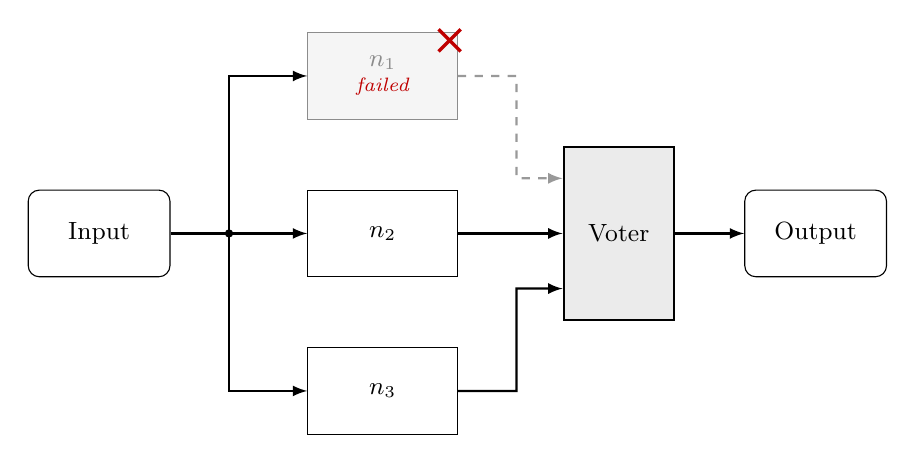
\begin{tikzpicture}[
      >=latex,
      font=\small,
      io/.style    ={draw, rounded corners=4pt, minimum width=1.8cm, minimum height=1.1cm},
      unit/.style  ={draw, minimum width=1.9cm, minimum height=1.1cm},
      failed/.style={unit, draw=black!45, text=black!45, fill=black!4},
      voter/.style ={draw, thick, fill=black!8, minimum width=1.4cm, minimum height=2.2cm,
                     align=center},
      wire/.style  ={draw, thick},
    ]
    % Nodes
    \node[io]   (in)  at (0,0)     {Input};
    \node[failed, align=center] (n1) at (3.6, 2.0)
      {$n_1$\\[-2pt]{\scriptsize\itshape\color{red!75!black} failed}};
    \node[unit] (n2)  at (3.6, 0)   {$n_2$};
    \node[unit] (n3)  at (3.6,-2.0) {$n_3$};
    \node[voter] (vot) at (6.6, 0)  {Voter};
    \node[io]   (out) at (9.1,0)   {Output};

    % Failure marker on n1: small red cross at the top-right corner
    \draw[red!75!black, very thick]
      ([shift={(-3pt,-3pt)}]n1.north east) ++(-4pt,-4pt) -- ++(8pt,8pt)
      ++(-8pt,0) -- ++(8pt,-8pt);

    % Fan-out from input to all three nodes
    \coordinate (split) at (1.65,0);
    \draw[wire] (in.east) -- (split);
    \draw[wire, ->] (split) |- (n1.west);
    \draw[wire, ->] (split) -- (n2.west);
    \draw[wire, ->] (split) |- (n3.west);
    \fill (split) circle (1.5pt);

    % Each node feeds its own voter input; n1 delivers no valid result
    \draw[wire, ->, dashed, black!40]
      (n1.east) -| (5.3, 0.7) -- ([yshift=0.7cm]vot.west);
    \draw[wire, ->] (n2.east) -- (vot.west);
    \draw[wire, ->]
      (n3.east) -| (5.3,-0.7) -- ([yshift=-0.7cm]vot.west);

    % Voter to output
    \draw[wire, ->] (vot.east) -- (out.west);
  \end{tikzpicture}

  \caption[TMR cluster with majority voter after failure of one node]{%
    Triple modular redundancy (TMR) cluster after the failure of node $n_1$.
    All three nodes receive the same input and feed their results to a
    majority voter. With $n_1$ failed, only $n_2$ and $n_3$ deliver results,
    so the cluster continues in degraded dual modular redundancy (DMR) mode:
    a disagreement between the two remaining nodes can still be detected,
    but no longer masked by a majority vote.}
  \label{fig:tmr-failure}
\end{figure}

% Needs only TikZ + the positioning library (already loaded via forest in main.tex)
\begin{figure}[htbp]
  \centering
  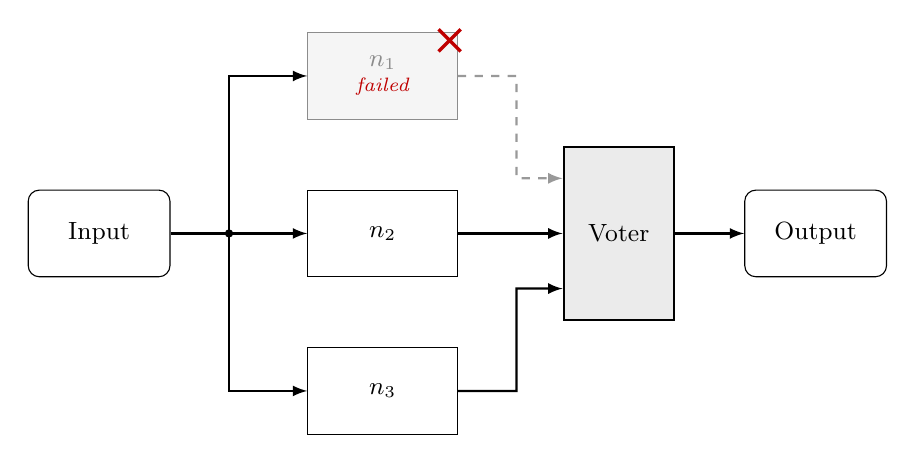
\begin{tikzpicture}[
      >=latex,
      font=\small,
      io/.style    ={draw, rounded corners=4pt, minimum width=1.8cm, minimum height=1.1cm},
      unit/.style  ={draw, minimum width=1.9cm, minimum height=1.1cm},
      failed/.style={unit, draw=black!45, text=black!45, fill=black!4},
      voter/.style ={draw, thick, fill=black!8, minimum width=1.4cm, minimum height=2.2cm,
                     align=center},
      wire/.style  ={draw, thick},
    ]
    % Nodes
    \node[io]   (in)  at (0,0)     {Input};
    \node[failed, align=center] (n1) at (3.6, 2.0)
      {$n_1$\\[-2pt]{\scriptsize\itshape\color{red!75!black} failed}};
    \node[unit] (n2)  at (3.6, 0)   {$n_2$};
    \node[unit] (n3)  at (3.6,-2.0) {$n_3$};
    \node[voter] (vot) at (6.6, 0)  {Voter};
    \node[io]   (out) at (9.1,0)   {Output};

    % Failure marker on n1: small red cross at the top-right corner
    \draw[red!75!black, very thick]
      ([shift={(-3pt,-3pt)}]n1.north east) ++(-4pt,-4pt) -- ++(8pt,8pt)
      ++(-8pt,0) -- ++(8pt,-8pt);

    % Fan-out from input to all three nodes
    \coordinate (split) at (1.65,0);
    \draw[wire] (in.east) -- (split);
    \draw[wire, ->] (split) |- (n1.west);
    \draw[wire, ->] (split) -- (n2.west);
    \draw[wire, ->] (split) |- (n3.west);
    \fill (split) circle (1.5pt);

    % Each node feeds its own voter input; n1 delivers no valid result
    \draw[wire, ->, dashed, black!40]
      (n1.east) -| (5.3, 0.7) -- ([yshift=0.7cm]vot.west);
    \draw[wire, ->] (n2.east) -- (vot.west);
    \draw[wire, ->]
      (n3.east) -| (5.3,-0.7) -- ([yshift=-0.7cm]vot.west);

    % Voter to output
    \draw[wire, ->] (vot.east) -- (out.west);
  \end{tikzpicture}

  \caption[TMR cluster with majority voter after failure of one node]{%
    Triple modular redundancy (TMR) cluster after the failure of node $n_1$.
    All three nodes receive the same input and feed their results to a
    majority voter. With $n_1$ failed, only $n_2$ and $n_3$ deliver results,
    so the cluster continues in degraded dual modular redundancy (DMR) mode:
    a disagreement between the two remaining nodes can still be detected,
    but no longer masked by a majority vote.}
  \label{fig:tmr-failure}
\end{figure}

% Needs only TikZ + the positioning library (already loaded via forest in main.tex)
\begin{figure}[H]
  \centering
  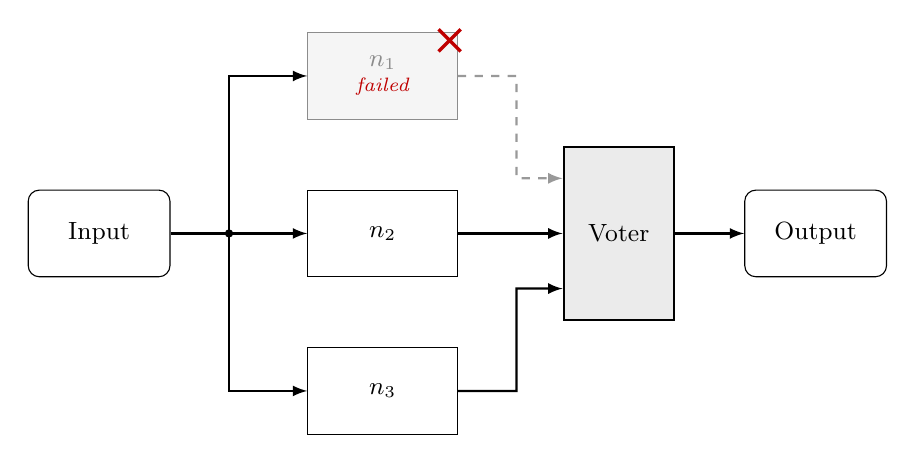
\begin{tikzpicture}[
      >=latex,
      font=\small,
      io/.style    ={draw, rounded corners=4pt, minimum width=1.8cm, minimum height=1.1cm},
      unit/.style  ={draw, minimum width=1.9cm, minimum height=1.1cm},
      failed/.style={unit, draw=black!45, text=black!45, fill=black!4},
      voter/.style ={draw, thick, fill=black!8, minimum width=1.4cm, minimum height=2.2cm,
                     align=center},
      wire/.style  ={draw, thick},
    ]
    % Nodes
    \node[io]   (in)  at (0,0)     {Input};
    \node[failed, align=center] (n1) at (3.6, 2.0)
      {$n_1$\\[-2pt]{\scriptsize\itshape\color{red!75!black} failed}};
    \node[unit] (n2)  at (3.6, 0)   {$n_2$};
    \node[unit] (n3)  at (3.6,-2.0) {$n_3$};
    \node[voter] (vot) at (6.6, 0)  {Voter};
    \node[io]   (out) at (9.1,0)   {Output};

    % Failure marker on n1: small red cross at the top-right corner
    \draw[red!75!black, very thick]
      ([shift={(-3pt,-3pt)}]n1.north east) ++(-4pt,-4pt) -- ++(8pt,8pt)
      ++(-8pt,0) -- ++(8pt,-8pt);

    % Fan-out from input to all three nodes
    \coordinate (split) at (1.65,0);
    \draw[wire] (in.east) -- (split);
    \draw[wire, ->] (split) |- (n1.west);
    \draw[wire, ->] (split) -- (n2.west);
    \draw[wire, ->] (split) |- (n3.west);
    \fill (split) circle (1.5pt);

    % Each node feeds its own voter input; n1 delivers no valid result
    \draw[wire, ->, dashed, black!40]
      (n1.east) -| (5.3, 0.7) -- ([yshift=0.7cm]vot.west);
    \draw[wire, ->] (n2.east) -- (vot.west);
    \draw[wire, ->]
      (n3.east) -| (5.3,-0.7) -- ([yshift=-0.7cm]vot.west);

    % Voter to output
    \draw[wire, ->] (vot.east) -- (out.west);
  \end{tikzpicture}

  \caption[TMR cluster with majority voter after failure of one node]{%
    Triple modular redundancy (TMR) cluster after the failure of node $n_1$.
    All three nodes receive the same input and feed their results to a
    majority voter. With $n_1$ failed, only $n_2$ and $n_3$ deliver results,
    so the cluster continues in degraded dual modular redundancy (DMR) mode:
    a disagreement between the two remaining nodes can still be detected,
    but no longer masked by a majority vote.}
  \label{fig:tmr-failure}
\end{figure}
